\documentclass[border=4mm,tikz]{standalone}
\usepackage[utf8]{inputenc}
\usepackage{pgfplots}
\usetikzlibrary{automata,positioning,arrows.meta}
\pgfplotsset{compat=1.15}
\tikzset{>={Latex[width=2mm,length=2mm]}}

\begin{document}
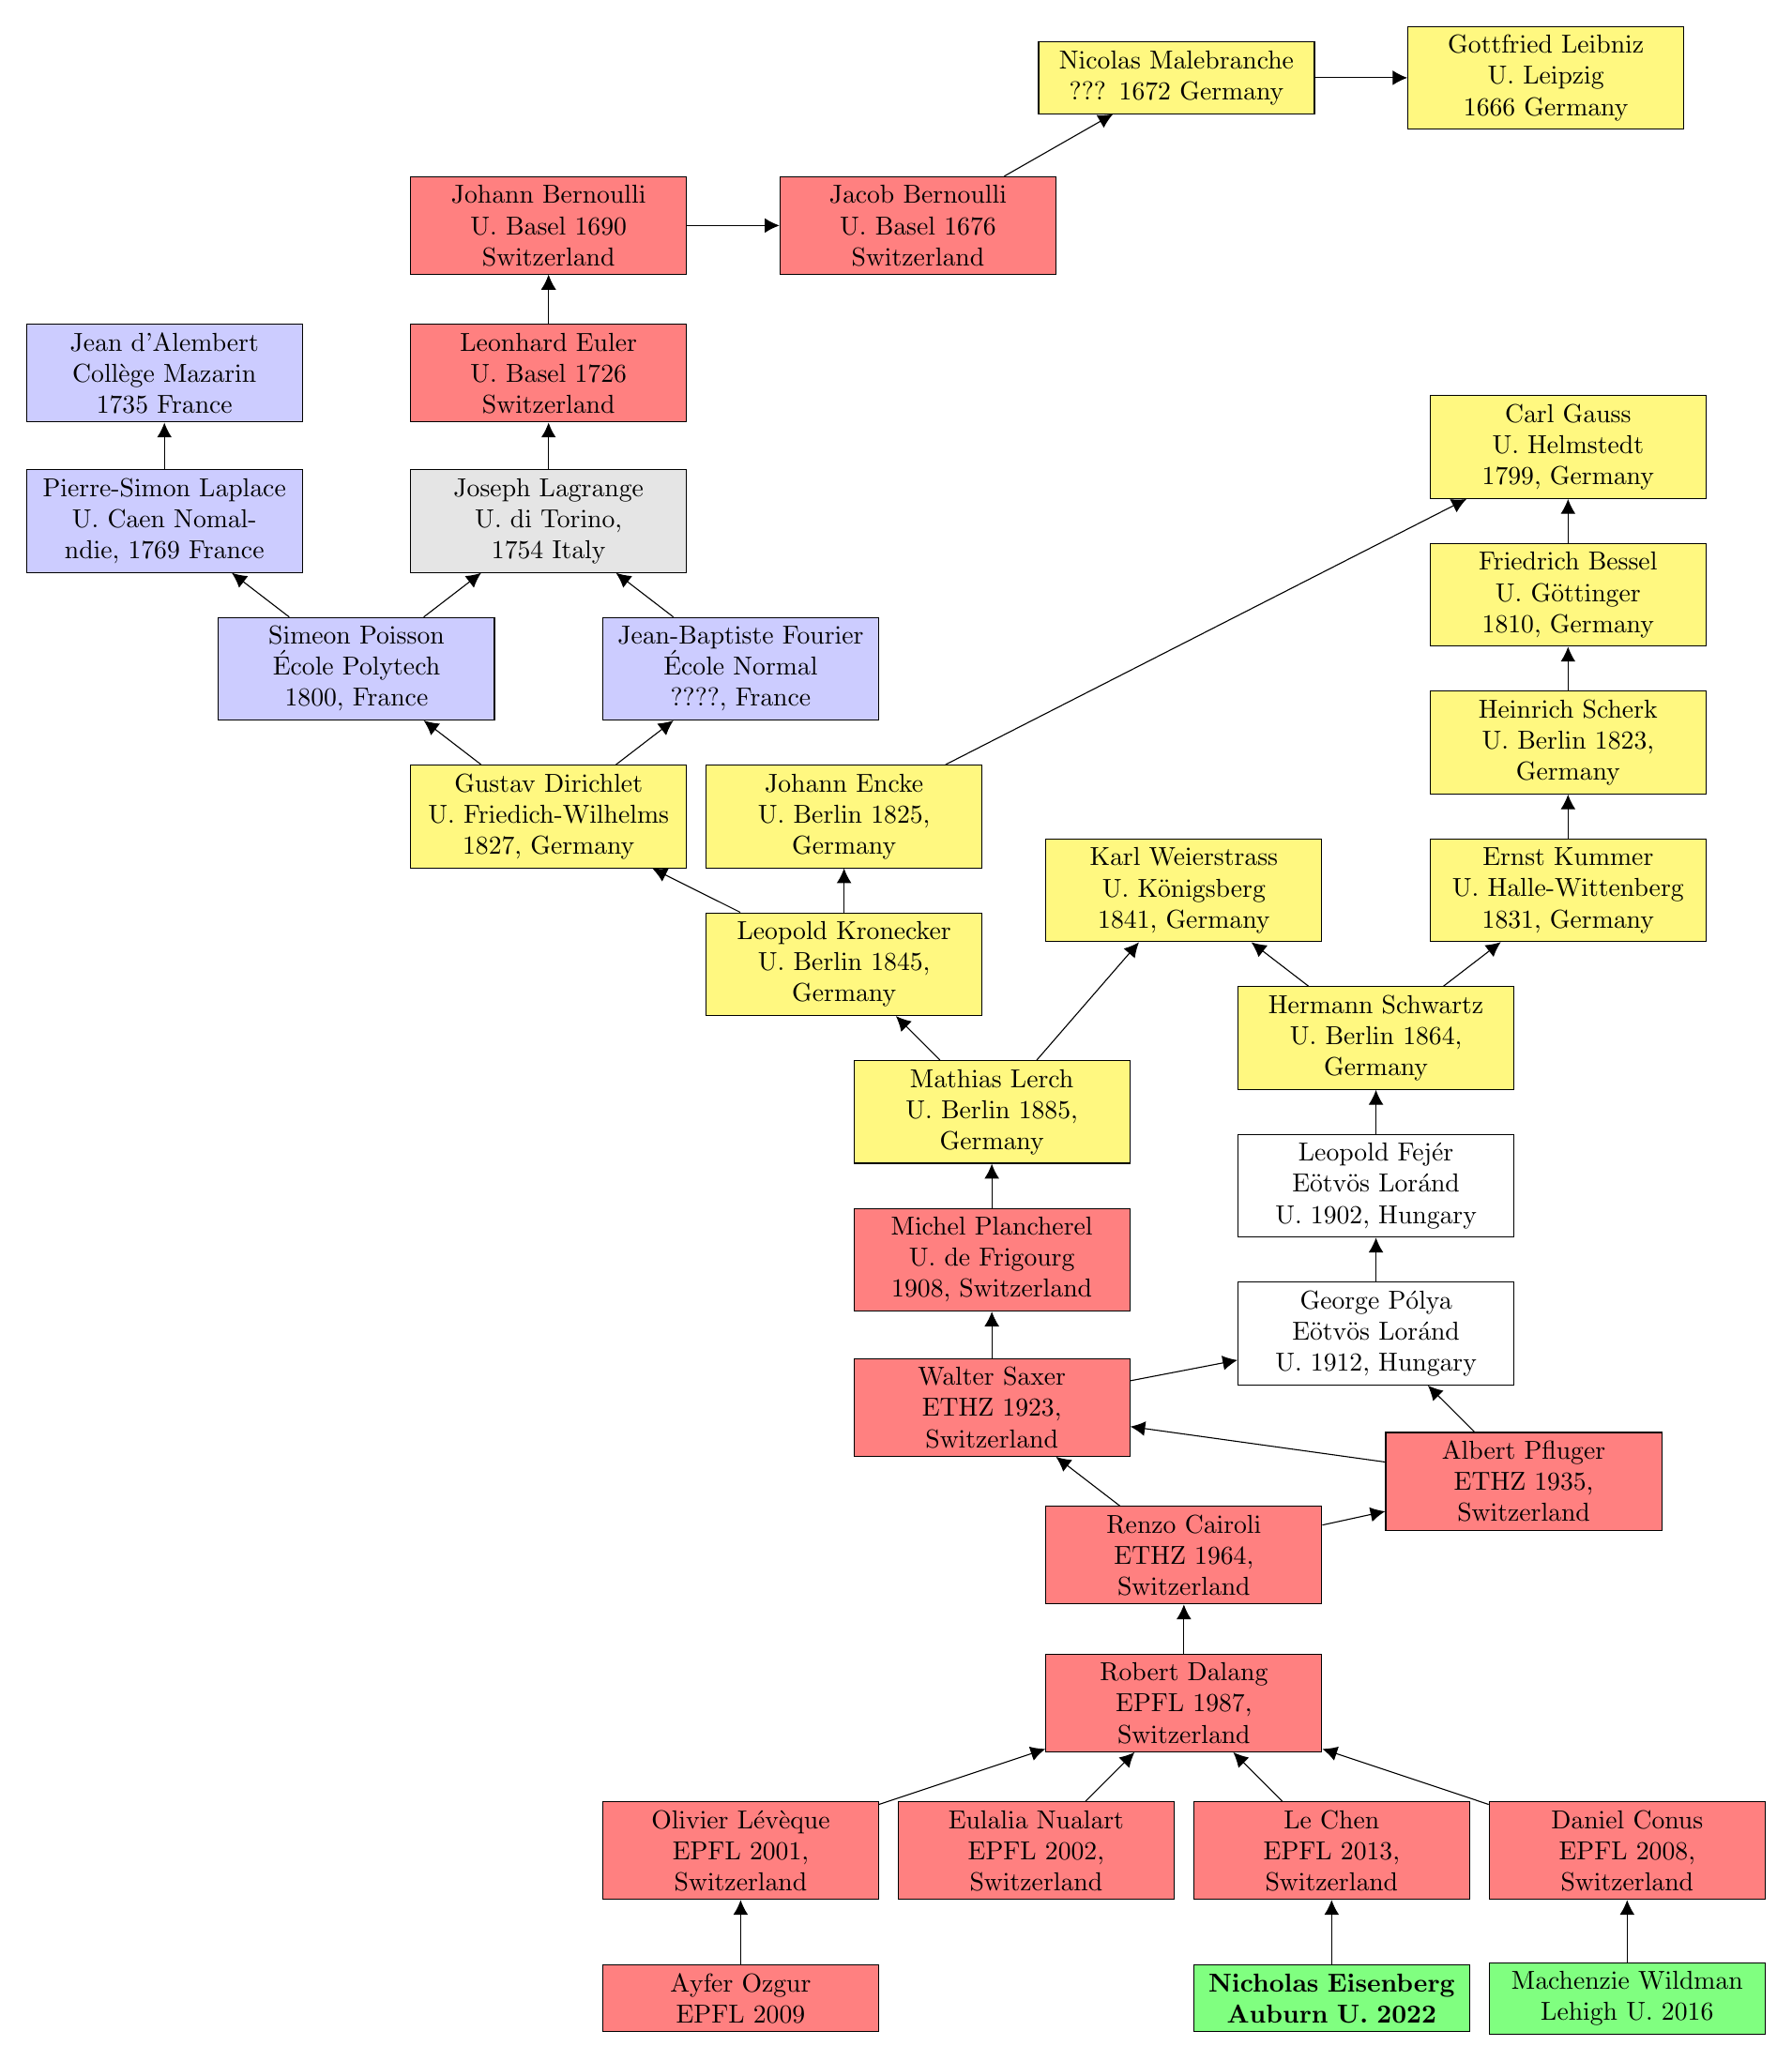
\begin{tikzpicture}[
    node distance=2cm,
  ]
  \node[fill = green!50, draw,text width=3.5cm, align = center] (Nick) at (0,0) {\bf Nicholas Eisenberg\\ Auburn U. 2022};
  \node[fill = red!50, draw,text width=3.5cm, align = center,above of = Nick] (Le) {Le Chen\\ EPFL 2013, Switzerland}; \draw[->] (Nick) -- (Le);
  \node[fill = red!50, draw,text width=3.5cm, align = center,above of = Le, xshift=-2cm] (Dalang) {Robert Dalang\\ EPFL 1987, Switzerland}; \draw[->] (Le) -- (Dalang);
  \node[fill = red!50, draw,text width=3.5cm, align = center,right of = Le, xshift=2cm] (Conus) {Daniel Conus\\ EPFL 2008, Switzerland}; \draw[->] (Conus) -- (Dalang);
  \node[fill = green!50, draw,text width=3.5cm, align = center,below of = Conus ] (Wildman) {Machenzie Wildman\\ Lehigh U. 2016}; \draw[->] (Wildman) -- (Conus);
  \node[fill = red!50, draw,text width=3.5cm, align = center,left of = Le,  xshift=-2cm] (Eulalia) {Eulalia Nualart\\ EPFL 2002, Switzerland}; \draw[->] (Eulalia) -- (Dalang);
  \node[fill = red!50, draw,text width=3.5cm, align = center,left of = Eulalia,  xshift=-2cm] (Leveque) {Olivier L\'ev\`eque\\ EPFL 2001, Switzerland}; \draw[->] (Leveque) -- (Dalang);
  \node[fill = red!50, draw,text width=3.5cm, align = center,below of = Leveque] (Ozgur) {Ayfer Ozgur\\ EPFL 2009}; \draw[->] (Ozgur) -- (Leveque);
  \node[fill = red!50, draw,text width=3.5cm, align = center,above of = Dalang] (Cairoli) {Renzo Cairoli\\ ETHZ 1964, Switzerland}; \draw[->] (Dalang) -- (Cairoli);
  \node[fill = red!50, draw,text width=3.5cm, align = center,above of = Cairoli, xshift = -2.6cm] (Saxer) {Walter Saxer\\ ETHZ 1923, Switzerland}; \draw[->] (Cairoli) -- (Saxer);
  \node[fill = red!50, draw,text width=3.5cm, align = center,above of = Cairoli, xshift = +4.6cm, yshift = -1cm] (Pfluger) {Albert Pfluger\\ ETHZ 1935, Switzerland}; \draw[->] (Cairoli) -- (Pfluger); \draw[->] (Pfluger)-- (Saxer);
  \node[fill = red!50, draw,text width=3.5cm, align = center,above of = Saxer] (Plancherel) {Michel Plancherel\\ U. de Frigourg 1908, Switzerland}; \draw[->] (Saxer) -- (Plancherel);
  \node[draw,text width=3.5cm, align = center,above of = Pfluger, xshift =-2cm] (Polya) {George P\'olya\\ E\"otv\"os Lor\'and U. 1912, Hungary}; \draw[->] (Pfluger) -- (Polya);
  \node[draw,text width=3.5cm, align = center,above of = Polya] (Fejer) {Leopold Fej\'er\\ E\"otv\"os Lor\'and U. 1902, Hungary}; \draw[->] (Saxer) -- (Polya) ; \draw[->] (Polya) -- (Fejer);
  \node[fill = yellow!50, draw,text width=3.5cm, align = center,above of = Fejer] (Schwartz) {Hermann Schwartz\\ U. Berlin 1864, Germany}; \draw[->] (Fejer) -- (Schwartz);
  \node[fill = yellow!50, draw,text width=3.5cm, align = center,above of = Schwartz, xshift =-2.6cm] (Weierstrass) {Karl Weierstrass\\ U. K\"onigsberg 1841, Germany}; \draw[->] (Schwartz) -- (Weierstrass);
  \node[fill = yellow!50, draw,text width=3.5cm, align = center,above of = Schwartz, xshift =+2.6cm] (Kummer) {Ernst Kummer\\ U. Halle-Wittenberg 1831, Germany}; \draw[->] (Schwartz) -- (Kummer);
  \node[fill = yellow!50, draw,text width=3.5cm, align = center,above of = Kummer] (Scherk) {Heinrich Scherk\\ U. Berlin 1823, Germany}; \draw[->] (Kummer) -- (Scherk);
  \node[fill = yellow!50, draw,text width=3.5cm, align = center,above of = Scherk] (Bessel) {Friedrich Bessel\\ U. G\"ottinger 1810, Germany}; \draw[->] (Scherk) -- (Bessel);
  \node[fill = yellow!50, draw,text width=3.5cm, align = center,above of = Bessel] (Gauss) {Carl Gauss\\ U. Helmstedt 1799, Germany}; \draw[->] (Bessel) -- (Gauss);

  \node[fill = yellow!50, draw,text width=3.5cm, align = center,above of = Plancherel] (Lerch) {Mathias Lerch\\ U. Berlin 1885, Germany}; \draw[->] (Plancherel) -- (Lerch); \draw[->] (Lerch) -- (Weierstrass);
  \node[fill = yellow!50, draw,text width=3.5cm, align = center,above of = Lerch, xshift=-2.0cm] (Kronecker) {Leopold Kronecker\\ U. Berlin 1845, Germany}; \draw[->] (Lerch) -- (Kronecker);

  \node[fill = yellow!50, draw,text width=3.5cm, align = center,above of = Kronecker, xshift=-0.0cm] (Encke) {Johann Encke\\ U. Berlin 1825, Germany}; \draw[->] (Kronecker) -- (Encke); \draw[->] (Encke) -- (Gauss);
  \node[fill = yellow!50, draw,text width=3.5cm, align = center,above of = Kronecker, xshift=-4.0cm] (Dirichlet) {Gustav Dirichlet\\ U. Friedich-Wilhelms 1827, Germany}; \draw[->] (Kronecker) -- (Dirichlet);
  \node[fill = blue!20, draw,text width=3.5cm, align = center,above of = Dirichlet, xshift=-2.6cm] (Poisson) {Simeon Poisson\\ \'Ecole Polytech 1800, France}; \draw[->] (Dirichlet) -- (Poisson);
  \node[fill = blue!20, draw,text width=3.5cm, align = center,above of = Dirichlet, xshift=+2.6cm] (Fourier) {Jean-Baptiste Fourier\\ \'Ecole Normal ????, France}; \draw[->] (Dirichlet) -- (Fourier);
  \node[fill = gray!20, draw,text width=3.5cm, align = center,above of = Poisson, xshift=+2.6cm] (Lagrange) {Joseph Lagrange\\ U. di Torino, 1754 Italy}; \draw[->] (Poisson) -- (Lagrange); \draw[->] (Fourier) -- (Lagrange);
  \node[fill = blue!20, draw,text width=3.5cm, align = center,above of = Poisson, xshift=-2.6cm] (Laplace) {Pierre-Simon Laplace\\ U. Caen Nomalndie, 1769 France}; \draw[->] (Poisson) -- (Laplace);
  \node[fill = blue!20, draw,text width=3.5cm, align = center,above of = Laplace] (dAlembert) {Jean d'Alembert\\ Coll\`ege Mazarin 1735 France}; \draw[->] (Laplace) -- (dAlembert);
  \node[fill = red!50, draw,text width=3.5cm, align = center,above of = Lagrange] (Euler) {Leonhard Euler\\ U. Basel 1726 Switzerland}; \draw[->] (Lagrange) -- (Euler);
  \node[fill = red!50, draw,text width=3.5cm, align = center,above of = Euler] (JohannB) {Johann Bernoulli\\ U. Basel 1690 Switzerland}; \draw[->] (Euler) -- (JohannB);
  \node[fill = red!50, draw,text width=3.5cm, align = center,right of = JohannB, xshift = 3cm] (Bernoulli) {Jacob Bernoulli\\ U. Basel 1676 Switzerland}; \draw[->] (Euler) -- (JohannB); \draw[->] (JohannB) -- (Bernoulli);
  \node[fill = yellow!50, draw,text width=3.5cm, align = center,above of = Bernoulli, xshift = 3.5cm] (Malebranche) {Nicolas Malebranche\\ ??? 1672 Germany}; \draw[->] (Bernoulli) -- (Malebranche);
  \node[fill = yellow!50, draw,text width=3.5cm, align = center,right of = Malebranche, xshift = 3cm] (Leibniz) {Gottfried Leibniz\\ U. Leipzig 1666 Germany}; \draw[->] (Malebranche) -- (Leibniz);

\end{tikzpicture}
\end{document}
